% !TEX options=--shell-escape
\documentclass[12pt]{article}
\usepackage[utf8]{inputenc}
\usepackage{lipsum}
\usepackage{afterpage}
\usepackage{mathtools}
\usepackage{xcolor}
\usepackage[12pt]{extsizes}
\usepackage[english,russian]{babel}
\usepackage{cite}
\usepackage{minted}
\usepackage{amsmath, esint, setspace, fancyhdr, amsfonts, bookmark, blindtext}
\usepackage{graphicx}
\usepackage{subfigure}
\usepackage{titlesec}

\graphicspath{{Figures/}}
\DeclareGraphicsExtensions{.pdf,.png,.jpg}
\usemintedstyle{tango}
\definecolor{dhscodebg}{rgb}{0.95,0.95,0.95}


\setlength{\textheight}{8in}
\setlength{\textwidth}{6.6in}
\setlength{\headheight}{0in}
\setlength{\headsep}{0.2in}
\setlength{\topmargin}{0in}
\setlength{\oddsidemargin}{0in}
\setlength{\evensidemargin}{0in}
\setlength{\parindent}{.3in}

\doublespacing
\renewcommand{\baselinestretch}{1.4} 
\newcommand{\RNumb}[1]{\uppercase\expandafter{\romannumeral #1\relax}}

\begin{document}
\begin{titlepage}

\begin{center}
Санкт-Петербургский политехнический университет Петра Великого\\
Институт прикладной математики и механики\\
Кафедра прикладной математики\\
\end{center}


\vspace{2.5cm}

\begin{center}
{\large {\bfseries СВОДНЫЙ ОТЧЕТ}}\\

\bigskip \bfseries{Тема:} {\bfseries \emph{Многомерные распределения.\\ Оценки характеристик распределений}}
\end{center}

\vspace{1.5cm}

\begin{flushleft}
Направление: 01.03.02 Прикладная математика и информатика

\vspace{1.5cm}

Выполнил студент гр. 33631/4 \hfill{Камалетдинова Ю.} \\ 

\vspace{0.5cm} Преподаватель \hfill{Баженов А.}
\vspace{1cm}

\end{flushleft}

\vspace{2.7cm}

\begin{center}
Санкт-Петербург\\
2019
\end{center}

\end{titlepage}

\newcommand{\threeimage}[4]{
\begin{figure}[h!]  
    \centering 
    \subfigure[]{
        \includegraphics[width=0.3\linewidth, height=0.25\linewidth]{#1} 
        \label{fig:f_ #1} }  
        %\hspace{4ex}
    \subfigure[]{
    \includegraphics[width=0.3\linewidth, height=0.25\linewidth]{#2} 
    \label{fig:f_ #2} }
   % \hspace{4ex}
    \subfigure[]{ 
        \includegraphics[width=0.3\linewidth, height=0.25\linewidth]{#3} 
        \label{fig:f_ #3} }  
    \caption{Выборки из #4 объемом: 
    \subref{fig:f_ #1} 20; 
    \subref{fig:f_ #2} 60; 
    \subref{fig:f_ #3} 100} 
    \label{fig:f_ #1#2#3}
\end{figure}}

\newcommand{\triplethreeimage}[4]{
\begin{figure}[h!]  
    \centering 
    \subfigure[]{
        \includegraphics[width=.83\linewidth, height=.3\linewidth]{#1} 
        \label{fig:f_ #1} }\\  
    %\hspace{4ex}
    \subfigure[]{
        \includegraphics[width=.83\linewidth, height=.3\linewidth]{#2} 
        \label{fig:f_ #2} }\\
    %\hspace{4ex}
    \subfigure[]{ 
        \includegraphics[width=.83\linewidth, height=.3\linewidth]{#2} 
        \label{fig:f_ #3} }  
    \caption{Для выборок из #4 объемом: 
    \subref{fig:f_ #1} 20; 
    \subref{fig:f_ #2} 60; 
    \subref{fig:f_ #3} 100} 
    \label{fig:f_ #1#2#3}
\end{figure}}


\tableofcontents
\addtocontents{toc}{~\hfill\par}
\vfill ~
\setcounter{section}{0}


%%%%%%%%%%%%%%%%%%%%%%%%%%%%%%%%%%%%%%%%%%

\newpage 
\section*{Постановка задачи}
\addcontentsline{toc}{section}{Постановка задачи}


\indent{\indentРассматривается линейная модель зависимости данных. Необходимо найти оценки коэффициентов линейной регрессии $y_i = a + bx_i + e_i$, используя $n = 20$ точек на отрезке $[-1.8; 2]$ с равномерным шагом равным 0.2. Ошибку $e_i$ считать нормально распределенной с параметрами (0, 1). В качестве эталонной зависимости взять функцию}
\begin{equation}
    \label{eq:1}
    y_i = 2 + 2x_i + e_i 
\end{equation}
\indent{При построении оценок коэффициентов использовать два критерия: критерий наименьших квадратов и критерий наименьших модулей. Требуется проделать описанную работу для выборки, у которой в значения $y_1$ и $y_{20}$ вносятся возмущения $10$ и $-10$.}

%%%%%%%%%%%%%%%%%%%%%%%%%%%%%%%%%%%%%%%%%%

\section*{Описание алгоритма}
\addcontentsline{toc}{section}{Описание алгоритма}
\subsection*{Метод наименьших квадратов}

\indent{\indent Введем обозначение для уравнения прямой, полученного по тому или иному критерию рассогласованности отклика и регрессионной модели}
\begin{equation}
    \label{eq:2}
    \hat y_i = \hat a + \hat bx_i ,
\end{equation}
где $\hat{a}, \hat{b}$ –– оценки параметров $a, b$

\indent{Запишем минимизируемое выражение для случая критерия наименьших квадратов (МНК)}
\begin{equation}
    \label{crit:1}
    Q(a, b) = \sum_{i=1}^{n}\epsilon^2 = \sum_{i=1}^{n}{(y_i - a - bx_i)^2} \rightarrow \underset{a, b} min
\end{equation}

\indent{Опустим запись необходимых условий экстремума и доказательства минимальности функции \eqref{crit:1} в стационарной точке, описанных в \cite{ms_1}, и приведем МНК-оценки коэффициентов}

\begin{equation}
    \label{coeff:1}
    \hat b = \frac{\overline{xy} - \overline{x} \cdot \overline {y}}{\overline{x^2} - (\overline{x})^2}
\end{equation}

\begin{equation}
    \label{coeff:2}
    \hat a = \overline{y} - \overline{x} \hat b,
\end{equation}

где $\overline{x}, \; \overline{x^2}, \; \overline{y}, \; \overline{xy}$ –– выборочные первые и вторые начальные моменты


\subsection*{Метод наименьших модулей}

\indent{\indent Одной из альтернатив МНК является метод наименьших модулей (МНМ)}
\begin{equation}
    \label{crit:2}
    A(a, b) = \sum_{i=1}^{n}{|y_i - a - bx_i|} \rightarrow \underset{a, b} min
\end{equation}

\indent{Запишем выражения для оценок \eqref{coeff:1}, \eqref{coeff:2} в другом виде}

\begin{equation}
    \label{coeff:3}
    \hat b = \frac{\overline{xy} - \overline{x} \cdot \overline {y}}{\overline{x^2} - (\overline{x})^2} = \frac{k_{xy}}{s_xs_y} = \frac{k_{xy}}{s^2_y} \frac{s_y}{s_x} = r_{xy} \frac{s_y}{s_x}
\end{equation}

\begin{equation}
    \label{coeff:4}
    \hat a = \overline{y} - \overline{x} \hat b,
\end{equation}

\indent{В формулах \eqref{coeff:3}, \eqref{coeff:4} заменим выборочные средние $\overline{x}, \; \overline{y}$ на выборочные медианы $med \; x, \; med \; y$, а среднеквадратические отклонения $s_x, \; s_y$ на интерквартильные широты $IQR_x, \; IQR_y$;  выборочный коэффициент корреляции $r_{xy}$ –– на знаковый коэффициент корреляции $r_Q$ }

\begin{equation}
    \label{coeff:5}
    \hat b_R = r_q \frac{IQR_y}{IQR_x},
\end{equation}

\begin{equation}
    \label{coeff:6}
    \hat a_R = med \; y - \hat b_R \; med \; x,
\end{equation}

\begin{equation}
    \label{coeff:7}
    r_Q = \frac{1}{n} \sum_{i=1}^{n}{sign(x_i - med \; x) \; sign(y_i - med \; y)}
\end{equation}

\begin{equation}
    \label{eq:3}
    sign \; z = 
    \begin{cases}
    \;\;\;1, \; z > 0 \\
    \;\;\;0, \; z = 0 \\
    -1, \;z < 0
    \end{cases}
\end{equation}

\indent{Формулы \eqref{coeff:3}, \eqref{coeff:4}, \eqref{coeff:5}, \eqref{coeff:6}, \eqref{coeff:7}, \eqref{eq:3} указаны в учебнике \cite{ms_1}. Уравнение регрессии примет вид}

\begin{equation}
    \label{eq:4}
    y = \hat a_R + \hat b_R x
\end{equation}
%%%%%%%%%%%%%%%%%%%%%%%%%%%%%%%%%%%%%%%%%%

\section*{Реализация}
\addcontentsline{toc}{section}{Реализация}
\indent{\indentДля выполнения поставленной задачи будем пользоваться библиотеками для языка Python: \textit{numpy, scipy} -- расчеты, законы распределения вероятностей; \textit{matplotlib, seaborn} -- визуализация результатов. Ход работы:}
\begin{itemize}
    \item Задаем вектор точек $x_n = [-1.8, -1.6, \ldots, 2.0]$ с шагом 0.2, $ \; n = 20$ 
    \item Вычисляем вектор значений функции \eqref{eq:1}
    \item Рассчитываем оценки коэффициентов линейной регрессии по формулам \eqref{coeff:1}, \eqref{coeff:2}, \eqref{coeff:5}, \eqref{coeff:6} 
    \item Вносим возмущения $+10$ и $-10$ в первое и последнее значения регрессионной функции соответсвтенно и повторяем шаги 2, 3
    \item Изображаем полученные результаты на графике и сравниваем коэффициенты, рассчитанные по разным критериям 
\end{itemize}

%%%%%%%%%%%%%%%%%%%%%%%%%%%%%%%%%%%%%%%%%%

\section*{Результат}
\addcontentsline{toc}{section}{Результат}
\begin{figure}[h!]

	\subfigure[]{
	\label{fig:1}
		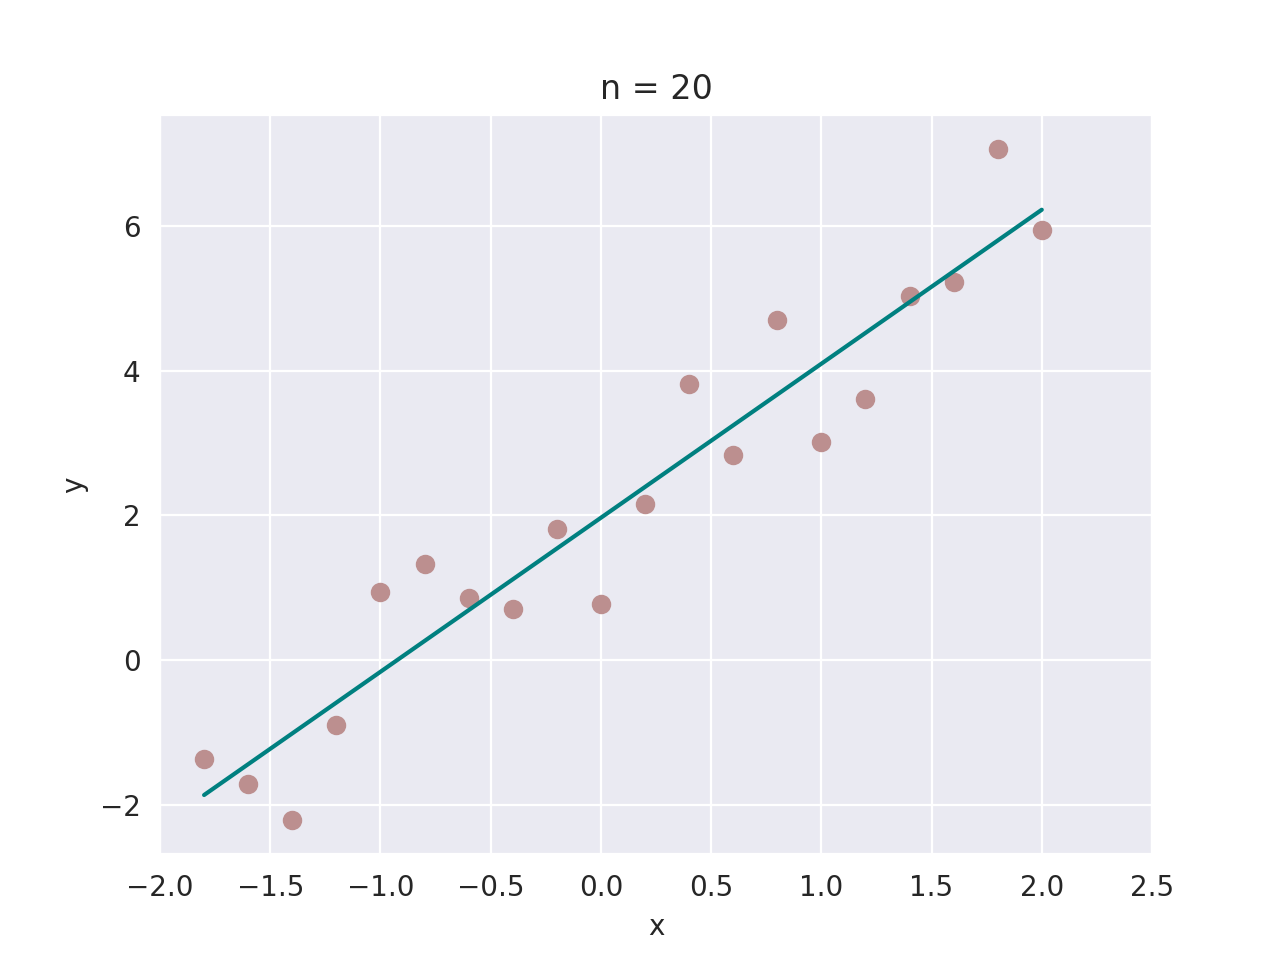
\includegraphics[width=0.5\linewidth, height=0.4\linewidth]{squares}} 
	\subfigure[]{
	\label{fig:2}
		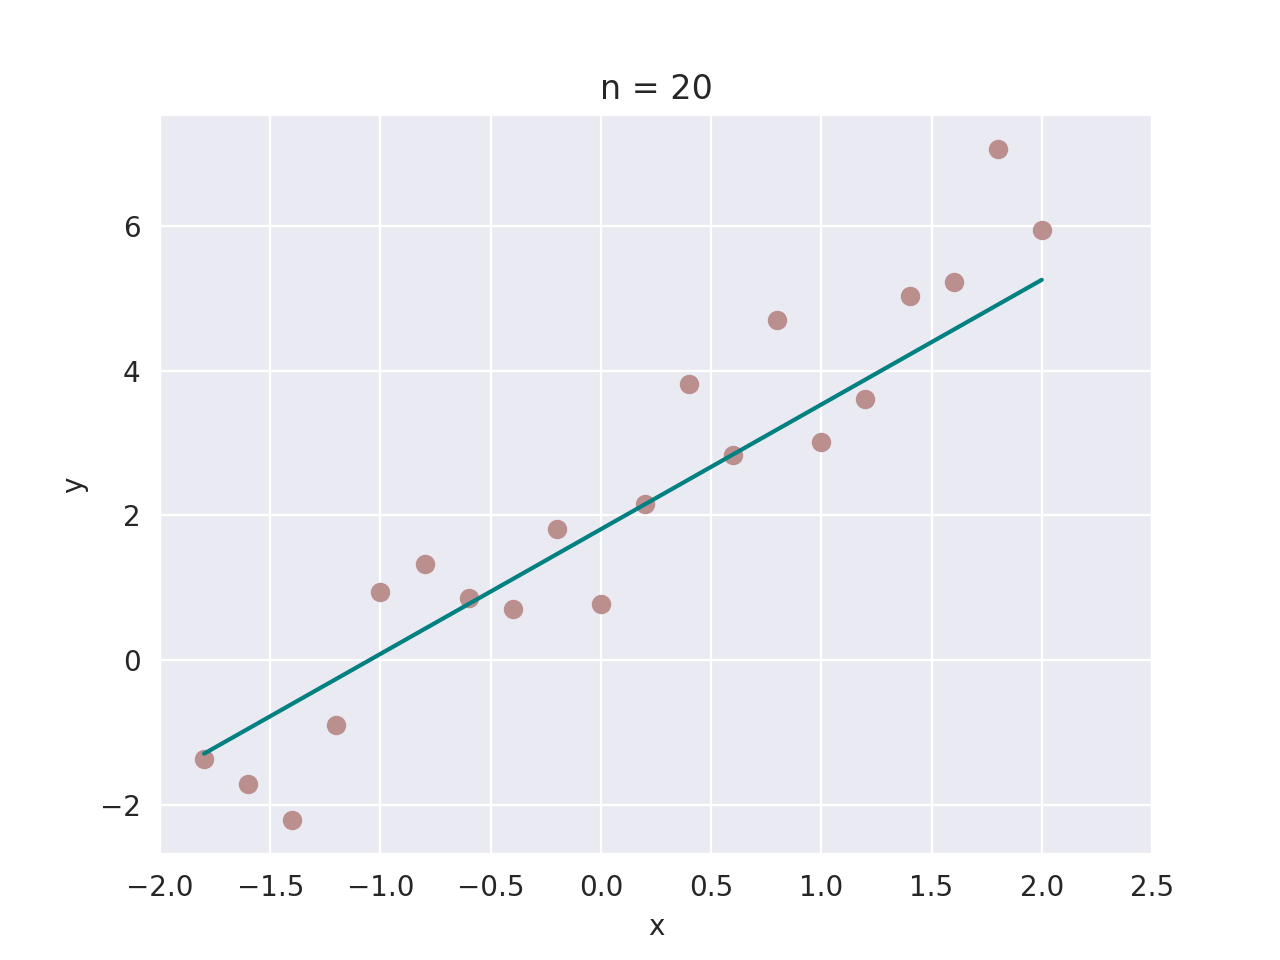
\includegraphics[width=0.5\linewidth, height=0.4\linewidth]{absolutes}}
	
	\caption{График прямой, исходные данные без возмущений
	\subref{fig:1} МНК; 
    \subref{fig:2} МНМ}
    \label{fig:1_2}
\end{figure}
\begin{multicols}{2}
    \raggedright
	\ref{fig:1}
	$\hat a = 1.9677, \; \hat b = 2.1254$

	\raggedleft
	\ref{fig:2}
	$\hat a = 1.8099, \; \hat b = 1.7207$
\end{multicols}
\vspace{10cm}
\begin{figure}[h!]
	\subfigure[]{
	\label{fig:3}
		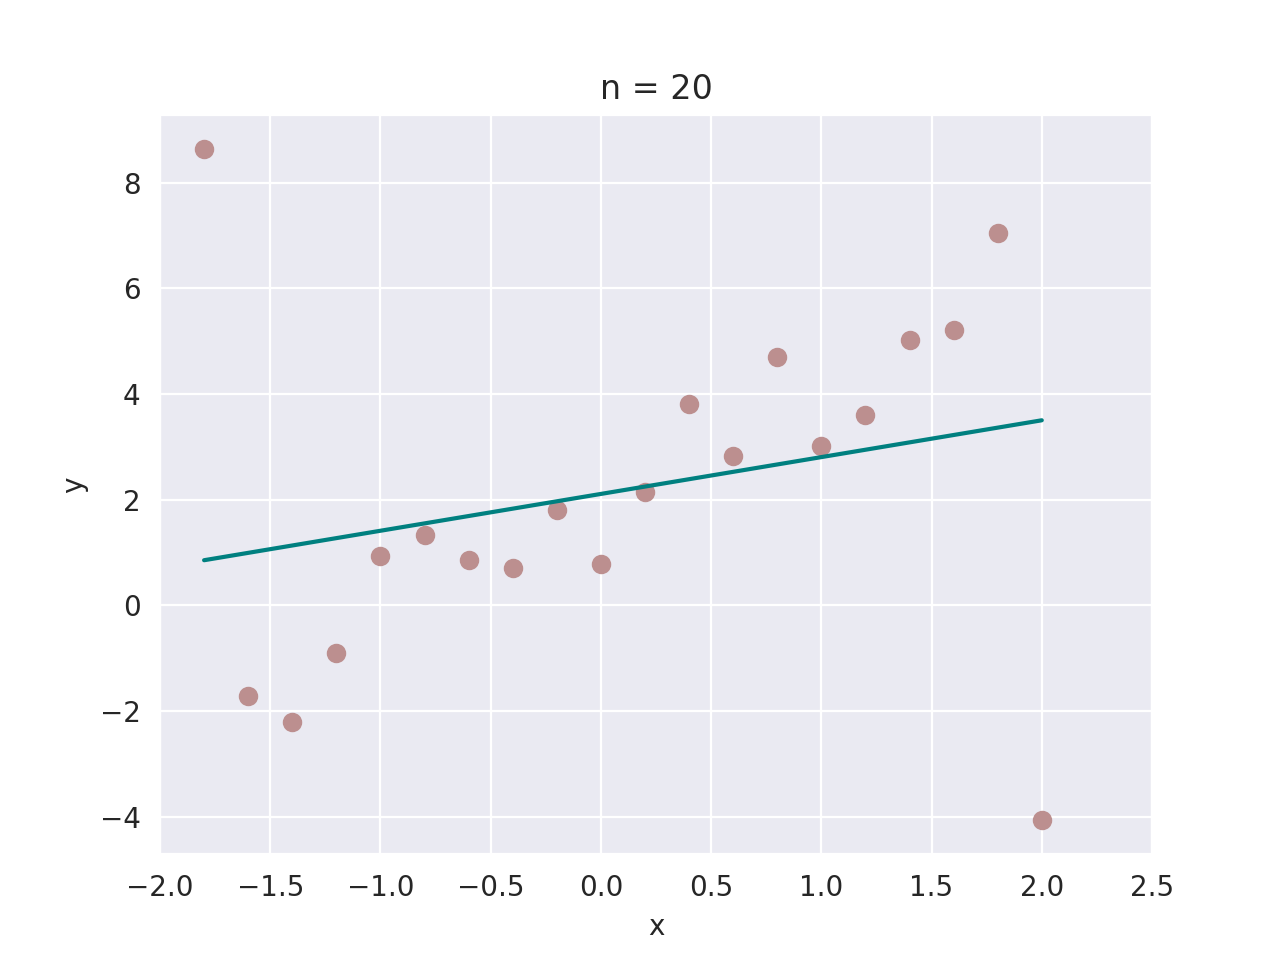
\includegraphics[width=0.5\linewidth, height=0.4\linewidth]{squares_err}} 
	\subfigure[]{
	\label{fig:4}
		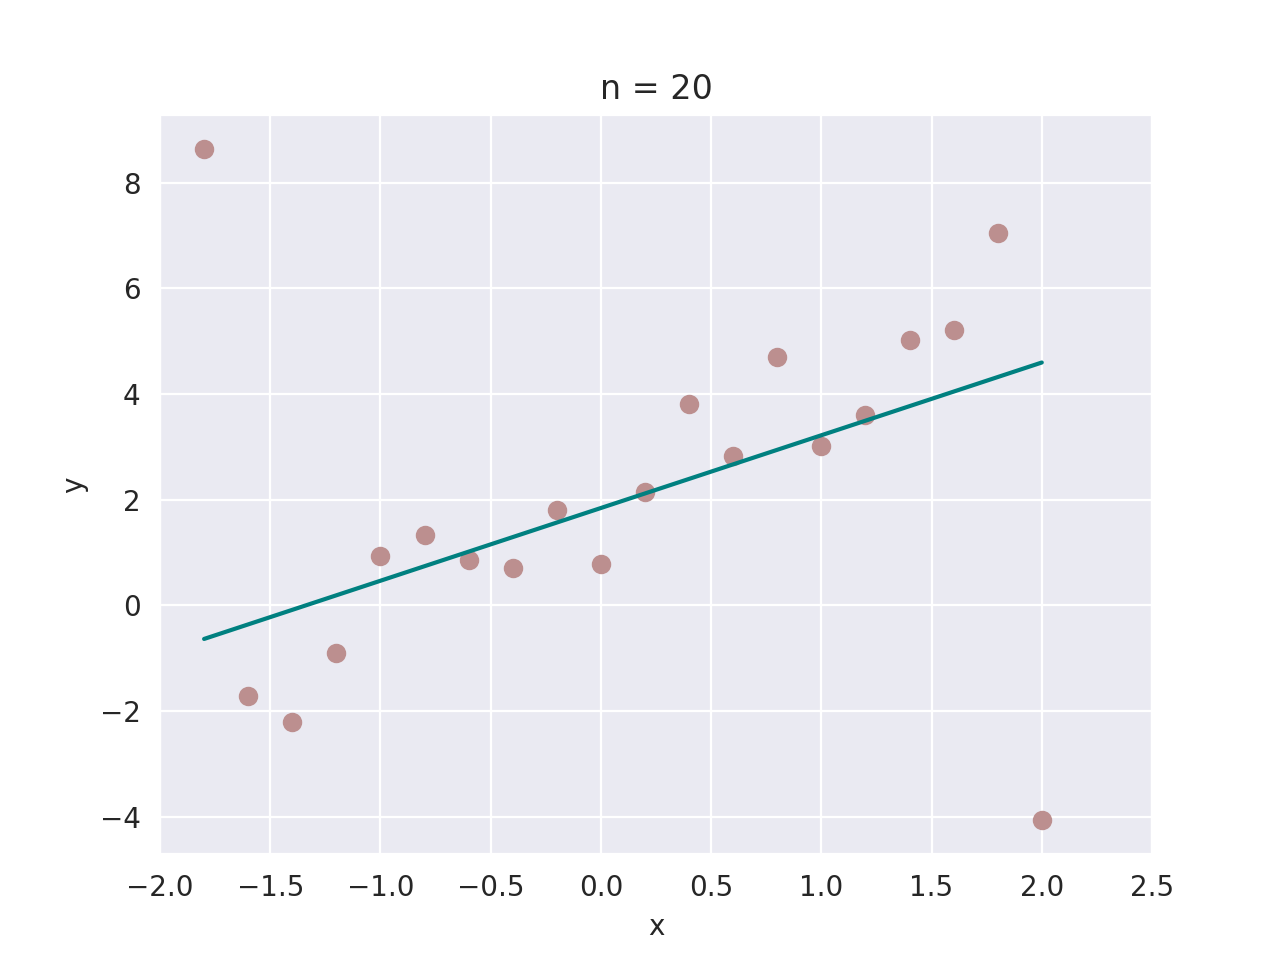
\includegraphics[width=0.5\linewidth, height=0.4\linewidth]{absolutes_err}}
	
	\caption{График прямой, исходные данные с возмущениями
	\subref{fig:3} МНК; 
    \subref{fig:4} МНМ}
    \label{fig:1_2}
\end{figure}
\begin{multicols}{2}
    \raggedright
	\ref{fig:3}
	$\hat a = 2.1106, \; \hat b = 0.6968$

	\raggedleft
	\ref{fig:4}
	$\hat a = 1.8443, \; \hat b = 1.3766$
\end{multicols}
\vspace{2cm}

\indent{ Результаты проведенной работы показывают, что наиболее устойчивым критерием к выбросам является метод наименьших модулей. Выборочная медиана и интерквартильные широты менее чувствительны к выбросам, что и объясняет полученные результаты.}

\indent{ Также можно заметить, что использование метода наименьших квадратов в случае отсутствия наблюдений, не свойственных данной выборке, дает лучшие результаты. Применение МНК при наличии больших по величине выбросов имеет смысл после предварительной отбраковки значений.}
%%%%%%%%%%%%%%%%%%%%%%%%%%%%%%%%%%%%%%%%%%

\newpage
\begin{thebibliography}{}
    \bibitem{ms_1}\textit{Амосова Н.Н., Куклин Б.А., Макарова С.Б., Максимов Ю.Д., Митрофанова Н.М., Полищук В.И., Шевляков Г.Л.} Вероятностные разделы математики. Учебник для бакалавров технических направлений. –– СПб.: Иван Федоров, 2001. –– 592 с.: илл. — ISBN 5-81940-050-X.
\end{thebibliography}


\end{document}{}